\documentclass[aspectratio=169]{beamer}
\usepackage[utf8]{inputenc}
\usepackage{graphicx}
\usepackage{listings}
\usepackage{xcolor}
\usepackage{tikz}
\usetikzlibrary{positioning,shapes,arrows}

% Theme
\usetheme{Madrid}
\usecolortheme{default}

% Colors
\definecolor{reactblue}{RGB}{0,122,255}
\definecolor{codegreen}{RGB}{52,199,89}
\definecolor{codegray}{RGB}{102,102,102}
\definecolor{codepurple}{RGB}{175,0,219}
\definecolor{backcolour}{RGB}{245,245,245}

% Code style - Simplified to avoid errors
\lstdefinestyle{mystyle}{
    backgroundcolor=\color{backcolour},
    commentstyle=\color{codegreen},
    keywordstyle=\color{reactblue},
    basicstyle=\ttfamily\footnotesize,
    breaklines=true,
    showspaces=false,
    showstringspaces=false
}

% Define JavaScript language for listings
\lstdefinelanguage{JavaScript}{
  keywords={const, let, var, function, return, if, else, for, while, import, export, default, from, class, extends, new, this, super},
  keywordstyle=\color{blue}\bfseries,
  ndkeywords={boolean, number, string, array, object},
  ndkeywordstyle=\color{darkgray}\bfseries,
  identifierstyle=\color{black},
  sensitive=false,
  comment=[l]{//},
  morecomment=[s]{/*}{*/},
  commentstyle=\color{purple}\ttfamily,
  stringstyle=\color{red}\ttfamily
}

\lstset{style=mystyle,language=JavaScript}

% Title Page
\title{React Native}
\subtitle{End-to-End Mobile Development}
\author{Mahima Kaushik}
\date{December 18, 2025}
\institute{2-Hour Comprehensive Session}

\begin{document}

% TITLE SLIDE
\begin{frame}
\titlepage
\end{frame}

% TABLE OF CONTENTS
\begin{frame}{Session Agenda}
\tableofcontents
\end{frame}

% SECTION 1: INTRODUCTION
\section{Introduction to React Native}

\begin{frame}{What is React Native?}
\begin{columns}
\column{0.5\textwidth}
\textbf{Definition:}
\begin{itemize}
    \item Framework for building mobile apps
    \item Uses JavaScript and React
    \item Created by Facebook (Meta) in 2015
    \item Write once, run on iOS \& Android
    \item Real native apps, not hybrid
\end{itemize}

\column{0.5\textwidth}
\textbf{Key Benefits:}
\begin{itemize}
    \item Cross-platform development
    \item Reuse web development skills
    \item Hot reload for fast iteration
    \item Large community support
    \item Native performance
\end{itemize}
\end{columns}

\vspace{0.5cm}
\begin{alertblock}{Analogy}
React Native is a translator - you speak JavaScript, it speaks Swift/Kotlin to the phone
\end{alertblock}
\end{frame}

\begin{frame}{How React Native Works}
\begin{center}
\textbf{The Bridge Architecture}
\end{center}

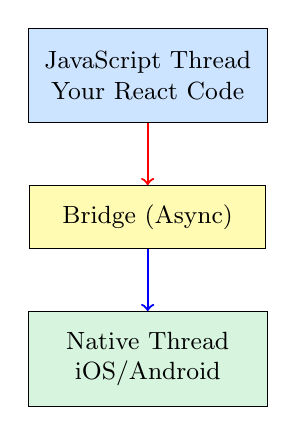
\begin{tikzpicture}[scale=0.9, every node/.style={font=\small}]
% JavaScript Thread
\node[draw, rectangle, fill=reactblue!20, minimum width=3cm, minimum height=1.2cm, text width=2.8cm, align=center] (js) at (0,4) {JavaScript Thread\\Your React Code};

% Bridge
\node[draw, rectangle, fill=yellow!30, minimum width=3cm, minimum height=0.8cm] (bridge) at (0,2) {Bridge (Async)};

% Native Thread
\node[draw, rectangle, fill=codegreen!20, minimum width=3cm, minimum height=1.2cm, text width=2.8cm, align=center] (native) at (0,0) {Native Thread\\iOS/Android};

\draw[->, thick, red] (js) -- (bridge);
\draw[->, thick, blue] (bridge) -- (native);
\end{tikzpicture}

\begin{block}{Key Concepts}
\begin{itemize}
    \item \textbf{Asynchronous:} Bridge is non-blocking
    \item \textbf{Batching:} Updates are batched for performance
    \item \textbf{Virtual DOM:} React calculates minimal changes
\end{itemize}
\end{block}
\end{frame}

\begin{frame}[fragile]{How It Works - Step by Step}
\begin{enumerate}
    \item \textbf{You write JSX:}
    \begin{lstlisting}
<View style={styles.container}>
  <Text>Hello!</Text>
</View>
    \end{lstlisting}

    \vspace{0.2cm}
    \item \textbf{React Native translates:}
    \begin{itemize}
        \item View → iOS: UIView / Android: ViewGroup
        \item Text → iOS: UILabel / Android: TextView
    \end{itemize}

    \vspace{0.2cm}
    \item \textbf{Bridge sends instructions} to native side
    \item \textbf{Native code renders} actual components
    \item \textbf{User interaction} → Event → Bridge → JavaScript
\end{enumerate}
\end{frame}

\section{What We Do With React Native}

\begin{frame}{Real-World Success Stories}
\begin{columns}
\column{0.5\textwidth}
\textbf{Apps Built with RN:}
\begin{itemize}
    \item Instagram (99\% shared code)
    \item Discord (60 FPS scrolling)
    \item Shopify (Complex features)
    \item Uber Eats (Real-time tracking)
    \item Facebook
    \item SoundCloud
\end{itemize}

\column{0.5\textwidth}
\textbf{When to Use RN:}
\begin{itemize}
    \item Cross-platform apps
    \item Rapid prototyping
    \item JavaScript team
    \item Frequent updates
\end{itemize}

\vspace{0.3cm}
\textbf{When NOT to use:}
\begin{itemize}
    \item Heavy 3D graphics/games
    \item Maximum performance critical
\end{itemize}
\end{columns}
\end{frame}

\section{Development Setup}

\begin{frame}[fragile]{Prerequisites \& Installation}
\begin{columns}
\column{0.5\textwidth}
\textbf{Required Software:}
\begin{itemize}
    \item Node.js (v16+)
    \item npm/npx
    \item Code editor (VS Code)
    \item Android Studio (for emulator)
\end{itemize}

\column{0.5\textwidth}
\textbf{Verify Installation:}
\begin{lstlisting}[language=bash]
node --version
npm --version
npx --version
\end{lstlisting}
\end{columns}

\vspace{0.5cm}
\begin{block}{Development Approaches}
\begin{itemize}
    \item \textbf{Expo} (Recommended): Managed workflow, quick setup
    \item \textbf{React Native CLI}: Full control, more complex
\end{itemize}
\end{block}
\end{frame}

\begin{frame}[fragile]{npm vs npx}
\begin{columns}
\column{0.5\textwidth}
\textbf{npm (Package Manager):}
\begin{lstlisting}[language=bash]
npm install package-name
npm install -g package-name
npm run start
\end{lstlisting}

\column{0.5\textwidth}
\textbf{npx (Package Executor):}
\begin{lstlisting}[language=bash]
npx create-expo-app MyApp
npx react-native init App
\end{lstlisting}
\end{columns}

\vspace{0.5cm}
\begin{block}{Why npx?}
\begin{itemize}
    \item No global installation needed
    \item Always uses latest version
    \item Saves disk space
\end{itemize}
\end{block}
\end{frame}

\section{Core Concepts}

\begin{frame}{Component Mapping: Web vs Native}
\begin{center}
\begin{tabular}{|l|l|}
\hline
\textbf{React (Web)} & \textbf{React Native} \\
\hline
div & View \\
span, p & Text \\
img & Image \\
input & TextInput \\
button & Button / TouchableOpacity \\
ul, li & FlatList \\
\hline
\end{tabular}
\end{center}

\vspace{0.5cm}
\begin{alertblock}{Key Difference}
No HTML in React Native! Everything is a React component.
\end{alertblock}
\end{frame}

\begin{frame}{React vs React Native}
\begin{center}
\begin{tabular}{|l|l|l|}
\hline
\textbf{Aspect} & \textbf{React (Web)} & \textbf{React Native} \\
\hline
Platform & Browsers & iOS \& Android \\
Elements & HTML tags & Native components \\
Styling & CSS files & StyleSheet objects \\
Layout & CSS Box Model & Flexbox (default) \\
Navigation & React Router & React Navigation \\
\hline
\end{tabular}
\end{center}

\vspace{0.5cm}
\textbf{Similarities:}
\begin{itemize}
    \item Same React principles (components, props, state, hooks)
    \item Same lifecycle methods
    \item JSX syntax
\end{itemize}
\end{frame}

\begin{frame}[fragile]{Styling in React Native}
\begin{columns}
\column{0.5\textwidth}
\textbf{No CSS Files!}
\begin{itemize}
    \item JavaScript objects
    \item StyleSheet.create()
    \item Flexbox by default
    \item No pixels
\end{itemize}

\column{0.5\textwidth}
\begin{lstlisting}
const styles = StyleSheet.create({
  container: {
    flex: 1,
    backgroundColor: '#fff',
    alignItems: 'center',
    justifyContent: 'center'
  }
});
\end{lstlisting}
\end{columns}

\vspace{0.5cm}
\begin{block}{Flexbox Properties}
flexDirection, justifyContent, alignItems, flex, padding, margin
\end{block}
\end{frame}

\section{Building Our Progressive App}

\begin{frame}{The Journey - One App, Four Versions}
\begin{center}
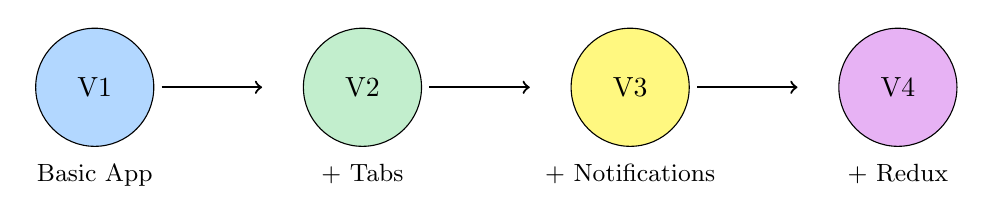
\begin{tikzpicture}[scale=0.85]
\node[draw, circle, fill=reactblue!30, minimum size=1.5cm] (v1) at (0,0) {V1};
\node[below=0.1cm of v1] {\small Basic App};

\draw[->, thick] (1,0) -- (2.5,0);

\node[draw, circle, fill=codegreen!30, minimum size=1.5cm] (v2) at (4,0) {V2};
\node[below=0.1cm of v2] {\small + Tabs};

\draw[->, thick] (5,0) -- (6.5,0);

\node[draw, circle, fill=yellow!50, minimum size=1.5cm] (v3) at (8,0) {V3};
\node[below=0.1cm of v3] {\small + Notifications};

\draw[->, thick] (9,0) -- (10.5,0);

\node[draw, circle, fill=codepurple!30, minimum size=1.5cm] (v4) at (12,0) {V4};
\node[below=0.1cm of v4] {\small + Redux};
\end{tikzpicture}
\end{center}

\vspace{0.5cm}
\textbf{Learning Path:}
\begin{enumerate}
    \item Start simple → Build foundation
    \item Add navigation → Multiple screens
    \item Add complexity → Real features
    \item Add state management → Scale up
\end{enumerate}
\end{frame}

\begin{frame}[fragile]{VERSION 1: Basic App}
\textbf{What We'll Build:}
\begin{itemize}
    \item Welcome screen with counter
    \item Buttons to increment/decrement
    \item Professional styling
\end{itemize}

\textbf{Concepts Covered:}
\begin{itemize}
    \item Components: View, Text, TouchableOpacity
    \item State: useState hook
    \item Events: onPress handlers
    \item Styling: StyleSheet.create, Flexbox
\end{itemize}

\vspace{0.3cm}
\begin{lstlisting}[language=bash]
npx create-expo-app MyApp
cd MyApp
npx expo start --android
\end{lstlisting}
\end{frame}

\begin{frame}[fragile]{VERSION 1: Key Code}
\begin{lstlisting}
import { useState } from 'react';
import { View, Text, TouchableOpacity } from 'react-native';

export default function App() {
  const [count, setCount] = useState(0);

  return (
    <View style={styles.container}>
      <Text>{count}</Text>
      <TouchableOpacity onPress={() => setCount(count + 1)}>
        <Text>+</Text>
      </TouchableOpacity>
    </View>
  );
}
\end{lstlisting}
\end{frame}

\begin{frame}{VERSION 1: Key Learnings}
\begin{block}{Components}
\begin{itemize}
    \item View is like div - a container
    \item Text for all text (required!)
    \item TouchableOpacity for touchable elements
\end{itemize}
\end{block}

\begin{block}{State}
\begin{itemize}
    \item useState() creates state variable
    \item State updates trigger re-render
    \item Always use setter function
\end{itemize}
\end{block}

\begin{block}{Styling}
\begin{itemize}
    \item StyleSheet.create() for optimization
    \item Camel case properties
    \item No units on numbers
\end{itemize}
\end{block}
\end{frame}

\begin{frame}[fragile]{VERSION 2: Adding Tab Navigation}
\textbf{Evolution:}
\begin{itemize}
    \item Keep counter from V1
    \item Add multiple screens
    \item Add bottom tab navigation
    \item Add icons for tabs
\end{itemize}

\textbf{Install Dependencies:}
\begin{lstlisting}[language=bash]
npm install @react-navigation/native @react-navigation/bottom-tabs
npx expo install react-native-screens react-native-safe-area-context
\end{lstlisting}

\textbf{Concepts Added:}
\begin{itemize}
    \item React Navigation setup
    \item NavigationContainer
    \item createBottomTabNavigator
    \item Screen components
\end{itemize}
\end{frame}

\begin{frame}{VERSION 2: Key Learnings}
\begin{block}{Navigation}
\begin{itemize}
    \item NavigationContainer wraps entire app
    \item Each screen is a separate component
    \item Tab navigator manages screen switching
    \item Icons change based on focused state
\end{itemize}
\end{block}

\begin{block}{Screen Organization}
\begin{itemize}
    \item Separate function for each screen
    \item Each screen has its own state
    \item Shared styles across screens
\end{itemize}
\end{block}
\end{frame}

\begin{frame}{VERSION 3: Adding Notifications}
\textbf{Evolution:}
\begin{itemize}
    \item Add Notifications tab
    \item List of notifications with FlatList
    \item Mark as read/unread
    \item Delete notifications
    \item Show unread count
\end{itemize}

\textbf{New Components:}
\begin{itemize}
    \item FlatList for efficient lists
    \item Alert API for confirmations
    \item Complex state (array of objects)
\end{itemize}

\textbf{Concepts Added:}
\begin{itemize}
    \item Lists and keys
    \item Array methods: map, filter
    \item Immutable state updates
\end{itemize}
\end{frame}

\begin{frame}{VERSION 3: Key Learnings}
\begin{block}{FlatList}
\begin{itemize}
    \item Use for long lists (not .map())
    \item renderItem function returns component
    \item keyExtractor for unique keys (required!)
    \item Virtualized - only renders visible items
\end{itemize}
\end{block}

\begin{block}{Immutable State Updates}
\begin{itemize}
    \item Don't mutate arrays directly
    \item Use spread operator: [...array, newItem]
    \item Use map() and filter() for updates
\end{itemize}
\end{block}
\end{frame}

\begin{frame}{VERSION 4: Props \& Redux}
\textbf{Final Evolution:}
\begin{itemize}
    \item Extract components with props
    \item Share state with Redux
    \item Connect all screens to store
    \item Global notification count
\end{itemize}

\textbf{Concepts Added:}
\begin{itemize}
    \item Props: passing data to components
    \item Redux store: centralized state
    \item useSelector: read from store
    \item useDispatch: send actions to store
\end{itemize}
\end{frame}

\begin{frame}{Props: Data Flow}
\begin{center}
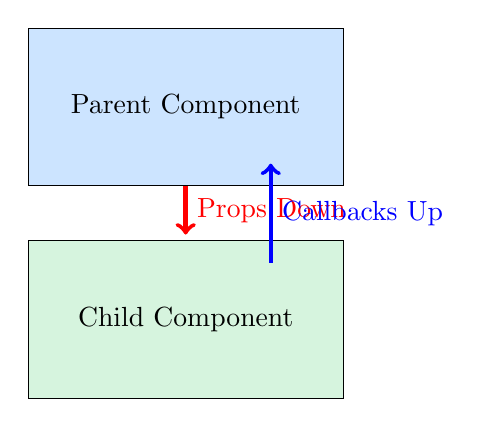
\begin{tikzpicture}[scale=0.9]
\node[draw, rectangle, fill=reactblue!20, minimum width=4cm, minimum height=2cm] (parent) at (0,3) {Parent Component};

\draw[->, ultra thick, red] (parent) -- (0,1.2) node[midway, right] {Props Down};

\node[draw, rectangle, fill=codegreen!20, minimum width=4cm, minimum height=2cm] (child) at (0,0) {Child Component};

\draw[->, ultra thick, blue] (1.2,0.8) -- (1.2,2.2) node[midway, right] {Callbacks Up};
\end{tikzpicture}
\end{center}

\begin{alertblock}{Remember}
\begin{itemize}
    \item Props flow DOWN (parent → child)
    \item Events flow UP (child → parent via callbacks)
    \item Props are READ-ONLY in child
\end{itemize}
\end{alertblock}
\end{frame}

\begin{frame}{Redux: When to Use}
\begin{columns}
\column{0.5\textwidth}
\textbf{Use Redux when:}
\begin{itemize}
    \item State shared across many components
    \item Complex state logic
    \item Large applications
\end{itemize}

\column{0.5\textwidth}
\textbf{Don't use if:}
\begin{itemize}
    \item Simple apps
    \item State in 1-2 components
    \item Can use Context API
\end{itemize}
\end{columns}
\end{frame}

\section{Best Practices}

\begin{frame}{Common Mistakes to Avoid}
\begin{block}{1. Mutating State Directly}
Wrong: items.push(newItem); setItems(items);\\
Correct: setItems([...items, newItem]);
\end{block}

\begin{block}{2. Missing Keys in Lists}
Wrong: items.map(item => <Item item={item} />)\\
Correct: items.map(item => <Item key={item.id} item={item} />)
\end{block}

\begin{block}{3. Inline Styling}
Wrong: style={{ flex: 1 }} (creates new object every render)\\
Correct: style={styles.container}
\end{block}
\end{frame}

\begin{frame}{Performance Tips}
\begin{enumerate}
    \item \textbf{Use FlatList} for long lists
    \item \textbf{Memoize} expensive components with React.memo
    \item \textbf{Optimize images} - resize before loading
    \item \textbf{Use StyleSheet.create()} - not inline styles
    \item \textbf{Profile} with React DevTools
\end{enumerate}
\end{frame}

\section{Swift Comparison}

\begin{frame}{Swift vs JavaScript: Overview}
\begin{center}
\begin{tabular}{|l|l|l|}
\hline
\textbf{Feature} & \textbf{JavaScript} & \textbf{Swift} \\
\hline
Type System & Dynamic & Static, strongly typed \\
Compilation & Interpreted (JIT) & Compiled (AOT) \\
Platform & Cross-platform & Apple only \\
Performance & Good & Excellent \\
Learning Curve & Easier & Steeper \\
\hline
\end{tabular}
\end{center}

\vspace{0.5cm}
\textbf{Key Difference:}
\begin{itemize}
    \item JavaScript: Flexible, dynamic, forgiving
    \item Swift: Strict, safe, explicit
\end{itemize}
\end{frame}

\begin{frame}{Why Learn Swift?}
\textbf{Swift is for:}
\begin{itemize}
    \item Native iOS development
    \item Maximum performance
    \item Full iOS platform access
    \item Official Apple language
\end{itemize}

\textbf{When you need Swift:}
\begin{itemize}
    \item iOS-specific features (Face ID, Apple Pay)
    \item Deep system integration
    \item Writing native modules for React Native
    \item Performance-critical code
\end{itemize}

\begin{alertblock}{Good News}
If you know JavaScript, Swift isn't that different!
\end{alertblock}
\end{frame}

\section{Conclusion}

\begin{frame}{What We Covered Today}
\begin{enumerate}
    \item Introduction to React Native
    \item How it works (Bridge architecture)
    \item Core Concepts (Components, Props, State)
    \item Built Progressive App (V1 → V2 → V3 → V4)
    \item Best Practices
    \item Swift Comparison
\end{enumerate}

\vspace{0.5cm}
\textbf{You've learned:}
\begin{itemize}
    \item Built 4 app versions
    \item Learned navigation
    \item Mastered state management
    \item Understood props and Redux
\end{itemize}
\end{frame}

\begin{frame}{Next Steps}
\begin{block}{Continue Learning}
\begin{itemize}
    \item Build a todo app from scratch
    \item Add features to progressive app
    \item Explore TypeScript
    \item Deploy to app stores
\end{itemize}
\end{block}

\begin{block}{Resources}
\begin{itemize}
    \item reactnative.dev
    \item docs.expo.dev
    \item reactnavigation.org
\end{itemize}
\end{block}

\begin{block}{Join Community}
\begin{itemize}
    \item React Native Discord
    \item Stack Overflow
    \item GitHub projects
\end{itemize}
\end{block}
\end{frame}

\begin{frame}{Project Ideas}
\textbf{Beginner:}
\begin{itemize}
    \item Todo List, Calculator, Weather app
\end{itemize}

\textbf{Intermediate:}
\begin{itemize}
    \item Chat app, E-commerce, Social feed
\end{itemize}

\textbf{Advanced:}
\begin{itemize}
    \item Real-time collaboration, Fitness tracker, Music player
\end{itemize}
\end{frame}

\begin{frame}{Thank You!}
\begin{center}
{\Huge Questions?}

\vspace{1cm}

\textbf{Contact:}\\
Email: mahima.kaushik@example.com

\vspace{1cm}

{\Large Keep Building!}
\end{center}
\end{frame}

\end{document}
